\chapter{基础知识}
\label{chap:preliminary}

\textit{本章介绍本文研究所需的信息论、博弈论及隐私保护的基本概念,包括Shannon信息论及其扩展,策略博弈、扩展博弈等博弈论概念,隐私分类及隐私保护基本模型。本章的内容主要为后文展开具体研究奠定基础。}
\section{Shannon信息论及其扩展}

\subsection{信息通信模型}
信息论\cite{shannon1948mathematical,
	stone2018information}是信息科学的基本工具,信息论对于量化信息的不确定性和信息量有重要的作用。信息通信模型最早由Shannon在其《通信的数学原理》论文中提出,如图\ref{fig:communication-model}所示。

\begin{figure}[htbp]
	\centering
	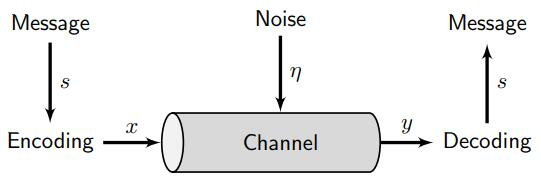
\includegraphics[width = 0.6\linewidth]{./figures/shannon-communicaiton-model.jpg}
	\caption{信息通信模型\cite{stone2018information}.
	}
	\label{fig:communication-model}
\end{figure}

信息通信模型\cite{stone2018information}由信源消息、编码器、信道、解码器、信宿消息和噪音构成,信源消息(数据)在作为信道输入之前被编码器进行编码;编码后的信源消息在信道中传输,传输过程中会受到噪声影响;解码器从信道中接收到加噪后的信息,解码为信宿消息。



对于事件集中的某一特定事件$x$,$x$的概率为$p(x)$,则$x$的香农信息为$-\text{log}p(x)$。

因此,风险也是关于不确定性的概念,这与香农信息自然相关。 在这项工作中,我们打算利用信息来估计访问请求和用户的隐私风险。 可以在\cite{wagner2018}中找到有关隐私社区中信息论的更多详细信息。

\subsection{信息熵}







\subsection{互信息}
\subsection{结构信息论}

\section{博弈论}
博弈论\cite{owen2001,gibbons1992} 是一个自我利益实体(即博弈者)之间相互作用的数学模型,它总是用于为这些实体寻找冲突与合作的解决方案。 博弈包含实体之间的迭代,并且每个博弈者在每次迭代中都将执行一个操作。 最后,博弈达到了解决方案(即平衡),所有博弈者都获得了自己最大的收益。 在特定的博弈中,博弈者是理性的,这意味着每个博弈者都会采取行动来响应他人的行动,以获取最大的利益。

有一些术语用来描述博弈、博弈者、行为、回报、策略和均衡\cite{liang2013}。博弈者是参与底层博弈的实体,博弈者可以是人、机构或信息系统;动作是每个博弈者在博弈的每个迭代中所做的动作,每个博弈者都知道每个其他博弈者的所有可选动作;博弈者的回报是对于他在博弈中采取的行动的返回值;博弈者的策略是他/她的行动计划,该计划根据他/她对行动历史的了解来指定要采取的行动。策略可以是纯策略,也可以是混合策略;均衡是一个博弈的解,是所有博弈者各自获得最大利益的策略组合。博弈论在信息安全和隐私保护的许多领域都得到了应用,详见\cite{liang2013,tian2019}。
\subsection{博弈模型}
\subsection{策略博弈}
\subsection{扩展博弈}
\subsection{演化博弈}


\section{隐私定义及隐私保护}
\subsection{身份隐私}
\subsection{属性隐私}
\subsection{隐私保护模型}

